\chapter{Identasi}
		\section{Pengertian Identasi} 
		Identasi adalah penulisan sebuah paragraf yang agak menjorong masuk kedalam. Pada python identasi digunakan untuk membuka atau menutup fungsi. Karena kode program python distrukturkan berdasarkan identasi. Identasi sangat mempengaruhi hasil eksekusi pada python.
		
		\section{Error pada Identasi} 
        Syntax Errors adalah suatu keadaan saat kode python mengalami kesalahan penulisan. Solusinya adalah memperbaiki penulisan kode yang salah.
        adapun error pada identasi sebagai berikut:
        \begin{enumerate}
            \item Python tidak menggunakan tanda { } untuk menandai blok / grup kode. Blok kode di python menggunakan tanda indentasi (spasi). Jumlah spasi untuk setiap baris yang ada dalam satu blok kode harus sama jika tidak maka akan terjadi error. Penulisan blok program harus ditambahkan indentasi (tab atau spasi 2x/4x).
            \begin{figure}[!htpb]
			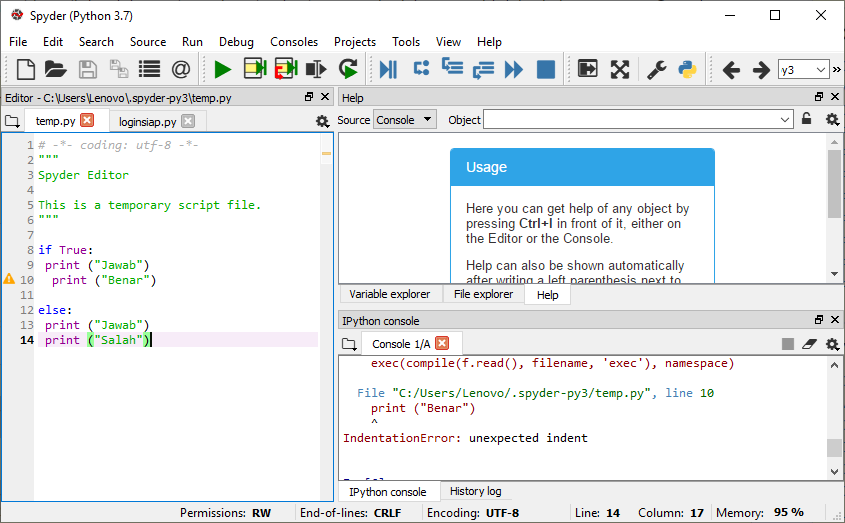
\includegraphics[width=10cm]{figures/identi2.PNG}
				\centering
			\caption{Error Pada Identasi}
		\end{figure}
        \end{enumerate}
        \newpage
        
        \section {Cara membaca Error yang ada pada Identasi}
        \begin{enumerate}
            \item Ketika programnya dijalankan dan mengalami error maka akan muncul pemberitahuan bahwa kodingan tersebut salah pada spasi (identasi) 
            \item Akan ada pemberitahuan segitiga kuning bertanda seru yang menandakan kodingan tersebut belum sepenuhnya benar
            \item jika ada error pada kodingan akan langsung diberitahukan letak linenya 
            \begin{figure}[!htpb]
			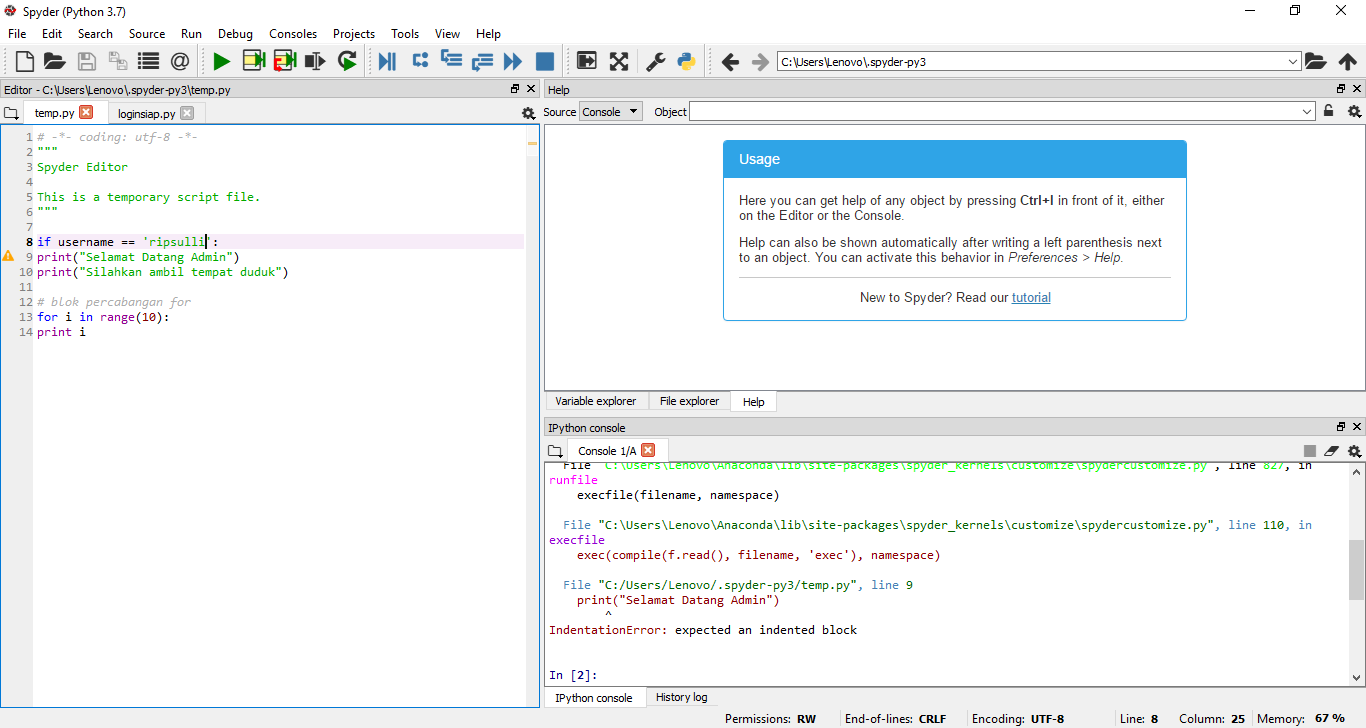
\includegraphics[width=10cm]{figures/identi1.PNG}
				\centering
			\caption{Pembertiahuan Error}
			\end{figure}
        \end{enumerate}
        
        \section{Cara menangani error}
            \begin{enumerate}
                \item Syntax Errors Syntax Errors adalah suatu keadaan saat kode python mengalami kesalahan penulisan. Solusinya adalah memperbaiki penulisan kode yang salah. Jika identasi nya salah dan muncul pemberitahuan error maka cek line ke berapa yang terjadapat error. Lalu lakukan perbaikan identasi (spasi) pada kodingan tersebut sampai tidak ada lagi error dan program dapat dijalankan.
                \item Zero Division Error ZeroDivisonError adalah exceptions yang terjadi saat eksekusi program menghasilkan perhitungan matematika pembagian dengan angka nol (0). Solusinya adalah tidak membagi suatu yang hasilnya nol.
                \item Name Error NameError adalah exception yang terjadi saat kode melakukaneksekusi terhadap local name atau global name yang tidak terdefinisi. Solusinya adalah memastikan variabel atau function yang dipanggil ada atau tidak salah ketik.
                \item Type Error TypeError adalah exception yang terjadi saat dilakukan eksekusi terhadap suatu operasi atau fungsi dengan type object yang tidak sesuai.Solusinya adalah mengkoversi varibelnya sesuai dengan tipe data yang akan digunakan.
            \end{enumerate}
